% File: state-space-cscw14-fig1.tex
\documentclass{standalone}

\usepackage{amssymb}
\usepackage{tikz}
\usetikzlibrary{shapes, positioning, arrows.meta, calc, backgrounds, fit, decorations.pathmorphing}

% default horizontal/vertical distance
\def\hdist{3.5}
\def\vdist{2.5}
\tikzset{node distance = \vdist and \hdist}

\newcommand{\ins}[2]{\textsc{Ins}(#1,#2)}
\newcommand{\del}[2]{\textsc{Del}(#1,#2)}
\newcommand{\set}[1]{\{#1\}}

\newcommand{\state}[3]{% #1: state name; #2: position; #3: state label
  \node (#1) [circle, inner sep = 0pt, minimum size = 8mm, text width = 8mm, align = center, draw, #2, font = \Large] {$#3$};
}
\newcommand{\lst}[3]{
  \node (#3) [rectangle, draw, #1 = 3pt of #2, font = \large] {$#3$};
}

\tikzset{path/.style = {>=Stealth, ->, decorate, decoration = {snake, post length = 1mm}}}
\tikzset{edge/.style = {>=Stealth, ->}}

\begin{document}
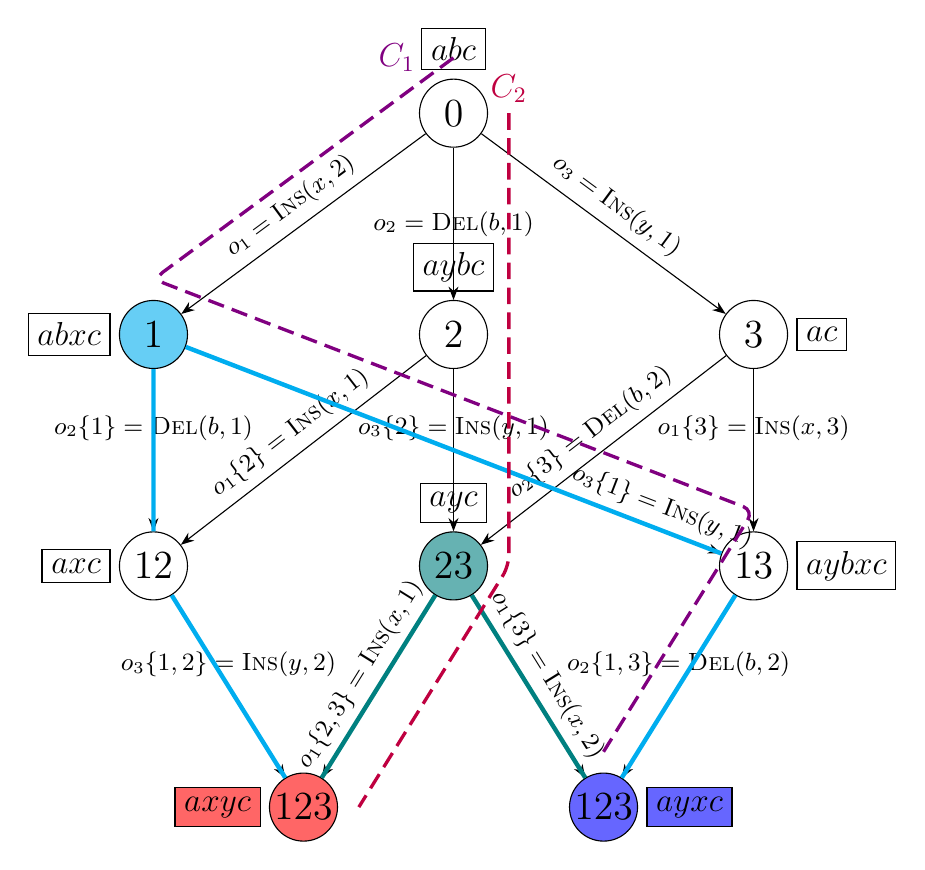
\begin{tikzpicture}
  % 1st level
  \state{0}{}{0}
  \lst{above}{0}{abc}
  % 2nd level
  \state{1}{below left = of 0.center, fill = cyan!60}{1}
  \lst{left}{1}{abxc}
  \state{3}{below right = of 0.center}{3}
  \lst{right}{3}{ac}
  \state{2}{at = ($(1)!0.50!(3)$)}{2}
  \lst{above}{2}{aybc}
  % 3rd level
  \state{12}{below = of 1.center}{12}
  \lst{left}{12}{axc}
  \state{23}{below = of 2.center, fill = teal!60}{23}
  \lst{above}{23}{ayc}
  \state{13}{below = of 3.center}{13}
  \lst{right}{13}{aybxc}
  % 4th level
  \node (c1) [at = ($(12)!0.50!(23)$)] {};
  \state{123l}{below = of c1, fill = red!60}{123}
  \node[left = 3pt of 123l, rectangle, draw, fill = red!60, font = \large] {$axyc$};
  \node (c2) [at = ($(23)!0.50!(13)$)] {};
  \state{123r}{below = of c2, fill = blue!60}{123}
  \node[right = 3pt of 123r, rectangle, draw, fill = blue!60, font = \large] {$ayxc$};

  \begin{scope}[trans/.style = {>=Stealth, ->},
	op/.style = {font = \small}]
    % 1st level -> 2nd level
    \draw[trans] (0) to node[op, sloped, above] {$o_1 = \ins{x}{2}$} (1);
    \draw[trans] (0) to node[op, ] {$o_2 = \del{b}{1}$} (2);
    \draw[trans] (0) to node[op, sloped, above] {$o_3 = \ins{y}{1}$} (3);
    % 2nd level -> 3rd level
	\draw[trans] (1) to node[op, above] {$o_2\set{1} = \del{b}{1}$} (12);
	\draw[trans] (1) to node[op, sloped, above, very near end] {$o_3\set{1} = \ins{y}{1}$} (13);
	\draw[trans] (2) to node[op, sloped, above] {$o_1\set{2} = \ins{x}{1}$} (12);
	\draw[trans] (2) to node[op, above] {$o_3\set{2} = \ins{y}{1}$} (23);
	\draw[trans] (3) to node[op, sloped, above] {$o_2\set{3} = \del{b}{2}$} (23);
	\draw[trans] (3) to node[op, above] {$o_1\set{3} = \ins{x}{3}$} (13);
	% 3rd level -> 4th level
	\draw[trans] (12) to node[op, above] {$o_3\set{1,2} = \ins{y}{2}$} (123l);
	\draw[trans] (23) to node[op, sloped, above] {$o_1\set{2,3} = \ins{x}{1}$} (123l);
	\draw[trans] (23) to node[op, sloped, above] {$o_1\set{3} = \ins{x}{2}$} (123r);
	\draw[trans] (13) to node[op, above] {$o_2\set{1,3} = \del{b}{2}$} (123r);
  \end{scope}
  
  \begin{scope}[lca/.style = {ultra thick}] % lca
	\draw[lca, cyan] (1) to (12) (12) to (123l) 
		(1) to (13) (13) to (123r);
	\draw[lca, teal] (23) to (123l) (23) to (123r);
  \end{scope}

  \def\dist{20pt}
  \begin{scope}[p/.style = {rounded corners, dash pattern = on 6pt off 3pt, very thick}] % path
	\draw[p, violet] ($(0.center)+(0,\dist)$) node[left = 10pt, font = \large] {$C_1$} 
		to[rounded corners] ($(1.center)+(0,\dist)$) to ($(13.center)+(0,\dist)$) to ($(123r.center)+(0,\dist)$);
	\draw[p, purple] ($(0.center)+(\dist,0)$) node[above, font = \large] {$C_2$} 
		to ($(2.center)+(\dist,0)$) to ($(23.center)+(\dist,0)$) to ($(123l.center)+(\dist,0)$);
  \end{scope}
\end{tikzpicture}
\end{document}
